\documentclass[10pt,t,usenames,dvipsnames]{beamer}

\usetheme{metropolis}   % Use metropolis theme

\usepackage{solarized}  % Use solarized themed listings

\ifnotes
  \hypersetup{final}
  \usepackage{pgfpages}
  \setbeamertemplate{note page}[plain]
  \setbeameroption{show notes on second screen=right}
  % the following fixes bug which causes normal text to be white instead of
  % template default when notes are enabled
  % (see https://tex.stackexchange.com/questions/232168/normal-text-is-invisible-when-using-beamer-with-notes-and-xelatex)
  \makeatletter 
  \def\beamer@framenotesbegin{% at beginning of slide
       \usebeamercolor[fg]{normal text}
        \gdef\beamer@noteitems{}% 
        \gdef\beamer@notes{}% 
  }
  \makeatother
\fi

\usepackage{appendixnumberbeamer}
\usepackage{tabularx}
\usepackage{listings}
\usepackage[scale=3]{ccicons}   % creative commons icons

%\newenvironment{termblock}%
%  {%
%    \setbeamercolor{block body}{bg=blue,fg=white}%
%    \begin{block}\begin{lstlisting}{language=bash}%
%  }{%
%    \end{lstlisting}\end{block}%
%  }

\title{C programming language}
\date{}
\author{Jeremy Iverson}
\institute{College of Saint Benedict \& Saint John's University}
\begin{document}
  \maketitle

  \begin{frame}{origins}
    \vspace{3ex}
    \begin{columns}
      \begin{column}{.38275\textwidth}
        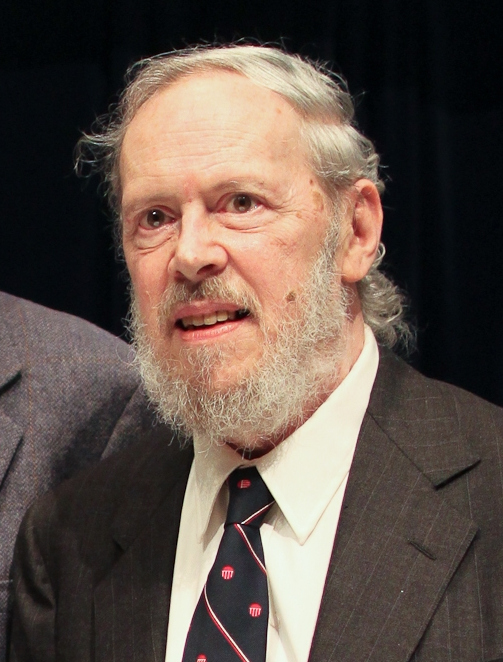
\includegraphics[width=\textwidth]{Dennis_Ritchie_2011.jpg}\\
        \hfill \tiny{\href{https://en.wikipedia.org/wiki/Dennis\_Ritchie\#/media/File:Dennis\_Ritchie\_2011.jpg}{Dennis~Ritchie~in~2011}~/~\href{http://creativecommons.org/licenses/by-sa/2.0}{CC~BY~2.0}}
      \end{column}
      \begin{column}{.51725\textwidth}
        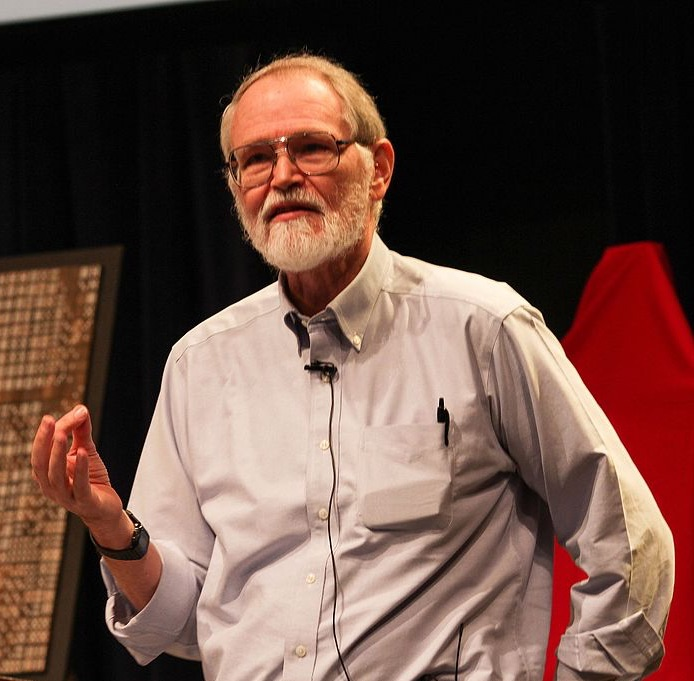
\includegraphics[width=\textwidth]{Brian_Kernighan_in_2012.jpg}\\
        \hfill \tiny{\href{https://en.wikipedia.org/wiki/Brian\_Kernighan\#/media/File:Brian\_Kernighan\_in\_2012\_at\_Bell\_Labs\_1.jpg}{Brian~Kernighan~in~2012}~/~\href{http://creativecommons.org/licenses/by-sa/2.0}{CC~BY~2.0}}
      \end{column}
    \end{columns}
  \end{frame}
  
  \begin{frame}{comparison}
    \begin{center}
      \begin{tabularx}{.8\textwidth}{XX}
        \hline
        \textbf{Java} & \textbf{C}\\
        \hline
        object-oriented & procedural\\
        interpreted & compiled\\
        \texttt{String} & \texttt{char} array\\
        condition (\texttt{boolean}) & condition (\texttt{int})\\
        garbage-collected & no memory management\\
        references & pointers\\
        exceptions & error codes\\
        \hline
      \end{tabularx}
    \end{center}

    \note{
      \begin{itemize}
        \item in Java, everything is a method that is called on an object
        \item in C, everything is a function
      \end{itemize}
      \begin{itemize}
        \item in Java, source code is compiled to byte code, which is then
          interpreted by Java VM
        \item in C, source code is compiled into binary machine code
      \end{itemize}
      \begin{itemize}
        \item in Java, String is a class
        \item in C, a string is just an array of \texttt{char} values which ends
          with the \texttt{char~'\textbackslash0'}
      \end{itemize}
      \begin{itemize}
        \item in Java, the Java VM takes care of deallocating memory used
        \item in C, any memory you allocate, you must also deallocate
      \end{itemize}
    }
  \end{frame}

  \begin{frame}[fragile]{hello, world}
    \begin{codeblock}
      ###include <stdio.h>##

      int main()
      {
        printf([["hello, world]]%%\n%%[["]]);
        return $$0$$;
      }
    \end{codeblock}

    \begin{termblock}
      $ gcc -o helloworld helloworld.c
      $ ./helloworld
      hello, world
    \end{termblock}
  \end{frame}

  \begin{frame}[fragile]{conditions}
    \begin{itemize}
      \item under what conditions will each of the following be execute?
    \end{itemize}
    \begin{codeblock}
      if (x) {
        /* ??? */
      }
      if (x-y) {
        /* ??? */
      }
      if (x=y) {
        /* ??? */
      }
    \end{codeblock}
  \end{frame}

  \begin{frame}{add evens}
    \begin{itemize}
      \item create program called \texttt{addEven.c} that adds all the even
        numbers between 1 and 100 and prints the sum
    \end{itemize}
  \end{frame}

  \begin{frame}[fragile]{add evens cont.}
    \begin{itemize}
      \item modify \texttt{addEven.c} to get maximum value from the command-line
        instead of hard-coded as 100
    \end{itemize}

    \begin{codeblock}
      ###include <stdio.h>##

      int main(int argc, char * argv[])
      {
        printf ([["(]]%%%d%%[[) ]]%%%s%%[[:]]%%%s\n%%[["]], argv[0], argv[1]);
        return $$0$$;
      } 
    \end{codeblock}
  \end{frame}

  \appendix

  \begin{frame}[c]
    \begin{center}\ccbysa\end{center}

    except where otherwise noted, this worked is licensed under
    \href{http://creativecommons.org/licenses/by-sa/4.0/}{creative commons
    attribution-sharealike 4.0 international license}
  \end{frame}
\end{document}
